\subsection{Progettazione Architetturale}
Periodo: dal 2020-01-22 al 2020-03-15\\
Inizia al termine della \glo{fase} di Analisi e finisce con la data di consegna per la Revisione di Progettazione.\\
In questa \glo{fase} viene definita una soluzione architetturale in modo da soddisfare i requisiti individuati nella \glo{fase} di Analisi.

\subsubsection{Periodo 1} 
Dal 2020-01-22 al 2020-02-20
\begin{itemize}
	\item \textbf{Normazione}: Standardizzazione e correzione di alcune parti della documentazione che non aderiscono completamente alle \NdP{};
	\item \textbf{\AdR{}}: Avvio della correzione e modifica dei casi d'uso segnalati, concentrandosi sui casi d'uso e requisiti segnalati (e non) utili al \glo{PoC};
	\item \textbf{Assegnazione dei ruoli di progetto}: Assegnazione dei ruoli di ciascun membro del gruppo in base alla suddivisione oraria indicata in §5.2.1;
	\item \textbf{Pianificazione delle attività}: Le attività da svolgere devono essere prima pianificate e discusse dal gruppo per garantire il \glo{way of working} sancito nelle \NdP{};
	\item \textbf{Approfondimento e studio delle tecnologie}: Ricerca di documentazione e materiali utili per l'apprendimento delle nuove tecnologie da utilizzare per la realizzazione del prodotto finale.
	In particolare:
	\begin{itemize}
		\item per l'app per gli utenti: il tool di build automation \glo{Gradle}, Java per Android, l'\glo{IDE} Android Studio, le \glo{API} di Google per Google Maps, Firebase, Google Play, il formato \glo{JSON}, la libreria client HTTP Volley;
		\item per la web-app per gli amministratori: il tool di build automation \glo{npm}, \glo{Node.js}, i framework \glo{Angular} e \glo{Bootstrap}, \glo{TypeScript};
		\item per il server: il tool di build automation Maven e i suoi \glo{plugin}, gli strumenti di \glo{Swagger} e lo standard \glo{OpenAPI}, il framework Spring per Java, il database \glo{Redis};
	\end{itemize}
	\item \textbf{Verifica}: \glo{Verifica} dell'andamento del team in relazione alle tempistiche e allo svolgimento dei compiti assegnati.
\end{itemize}
\paragraph{Milestone sull'ITS di GitHub}
\begin{itemize}
	\item \href{https://github.com/qb-team/Stalker-Documentazione/milestone/8}{Documentazione}.
\end{itemize}

\subsubsection{Periodo 2} 
Dal 2020-02-21 al 2020-03-02
\begin{itemize}
	\item \textbf{Approfondimento delle tecnologie}: \glo{LDAP}, \glo{GPS} per l'app per gli utenti, \glo{Angular} e \glo{Bootstrap} per la web-app per gli amministratori, Spring, \glo{Swagger} e \glo{Redis} per il server;
	\item \textbf{Normazione}: Decisioni ed inserimento delle nuove regole da adottare per le attività di progettazione e sviluppo;
	\item \textbf{Incrementi}: Nella sezione §3.3 sono stati elencati i requisiti sotto forma di incrementi che seguiti in successione portano al prodotto che soddisfa le richieste degli \glo{stakeholder}.
	In questo periodo viene portato avanti un incremento detto "\textit{Incremento 0}" che ha lo scopo, una volta completato, di fornire una base per il prodotto che deve essere realizzato, facendo comprendere al proponente e al committente
	il modo in cui il gruppo sta lavorando e al gruppo se il proprio \glo{way of working} è buono o va migliorato per poter realizzare con \glo{efficacia} anche i punti più critici del prodotto richiesto;
	\item \textbf{Progettazione}: Ricerca di una soluzione soddisfacente per tutti gli \glo{stakeholder}, che descriva l'architettura del prodotto prima di pensare al codice, seguendo gli incrementi definiti.
	La definizione dell'architettura deve essere proposta al proponente per ricevere feedback sulla sua bontà;
	\item \textbf{Technology Baseline}: Base per la realizzazione del \glo{Proof of Concept} nell'immediato e della \glo{Product Baseline} successivamente, che dimostra le tecnologie (librerie, framework, linguaggi) selezionate per lo sviluppo del prodotto;
	\item \textbf{Proof of Concept}: Creazione di uno più eseguibili che permettano di dimostrare la validità del prodotto che si vuole fornire, concretizzando la \glo{Technology Baseline}.
	Il \glo{Proof of Concept} realizzato è composto di:
	\begin{itemize}
		\item un'app per utenti sviluppata per dispositivi Android, che fornisca le funzionalità di autenticazione e logout, scaricamento della lista delle organizzazioni, verifica di presenza o meno all'interno dell'\glo{organizzazione} e visionare lo storico degli accessi;
		\item una web-app per amministratori che fornisca le funzionalità di autenticazione e logout, scaricamento della lista delle organizzazioni, visualizzazione delle informazioni di un'\glo{organizzazione}, controllo del numero di utenti presenti all'interno dell'\glo{organizzazione};
		\item un server che permetta all'app e alla web-app di ottenere i dati per fornire a utenti e amministratori rispettivamente le funzionalità richieste.
	\end{itemize}
	\item \textbf{Codifica}: Viene codificato il \glo{Proof of Concept} e successivamente condiviso tramite i \glo{repository} del gruppo al committente e al proponente per il colloquio TB in data 3 marzo;
	\item \textbf{Verifica}: \glo{Verifica} dell'andamento del gruppo in relazione alle tempistiche e allo svolgimento dei compiti assegnati.
\end{itemize}
\paragraph{Milestone sull'ITS di GitHub}
\begin{itemize}
	\item \href{https://github.com/qb-team/Stalker-Documentazione/milestone/9}{Documentazione}.
\end{itemize}

\subsubsection{Periodo 3} 
Dal 2020-03-03 al 2020-03-08
\begin{itemize}
	\item \textbf{Miglioramento standard di qualità}: Aggiunta, rimozione o modifica di alcune metriche per garantire le qualità di \glo{processo} e di prodotto affermate nel \PdQ{};
	\item \textbf{\AdR{}}: Continuazione della correzione del documento alla luce della correzione e del colloquio con il committente in data 2020-02-18;
	\item \textbf{Verifica}: \glo{Verifica} dell'andamento del gruppo in relazione alle tempistiche e allo svolgimento dei compiti assegnati.
\end{itemize}
\paragraph{Milestone sull'ITS di GitHub}
\begin{itemize}
	\item \href{https://github.com/qb-team/Stalker-Documentazione/milestone/10}{Documentazione}.
\end{itemize}

\subsubsection{Periodo 4} 
Dal 2020-03-09 al 2020-03-15
\begin{itemize}
	\item \textbf{Consolidamento}: Ogni membro si prende del tempo per ripassare tutto il lavoro svolto e per studiare il necessario per affrontare al meglio le \glo{fasi} successive;
	\item \textbf{Avvio allo studio delle tecnologie mancanti}: Prima dell'avvio della successiva \glo{fase}, cominciare lo studio delle tecnologie non impiegate per il \glo{Proof of Concept} ma necessarie per il prodotto;
	\item \textbf{Preparazione per la Revisione di Progettazione}: Il gruppo produce il materiale necessario da esporre alla presentazione pubblica della propria proposta.
\end{itemize}
\paragraph{Milestone sull'ITS di GitHub}
\begin{itemize}
	\item \href{https://github.com/qb-team/Stalker-Documentazione/milestone/14}{Documentazione}.
\end{itemize}

%PAGINA ORIZZONTALE
\newpage
\paperwidth=\pdfpageheight
\paperheight=\pdfpagewidth
\pdfpageheight=\paperheight
\pdfpagewidth=\paperwidth
\headwidth=\textheight

\begingroup 
\vsize=\textwidth
\hsize=\textheight

\subsubsection{Diagramma di Gantt delle attività della fase di Progettazione Architetturale}
\pagestyle{empty}
\begin{figure}[h]
	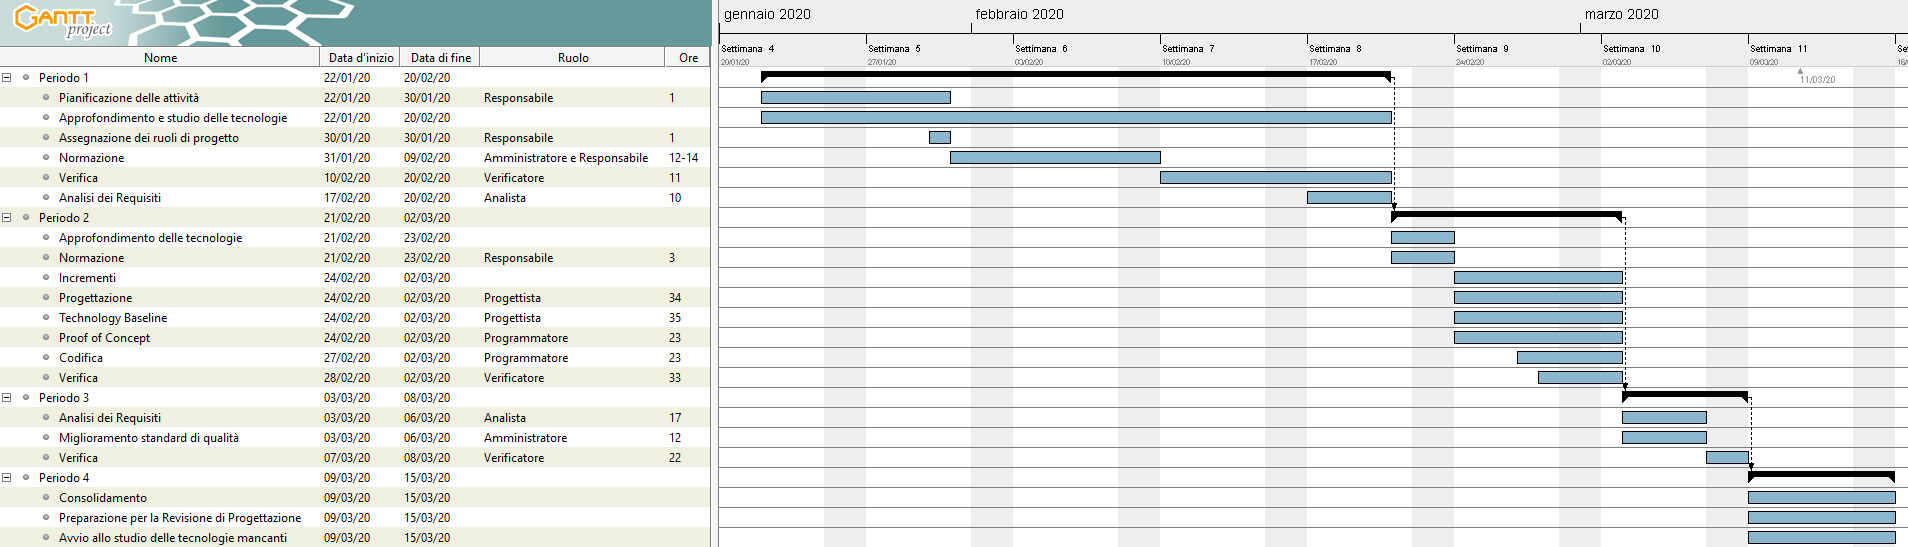
\includegraphics[height = 10cm, width = 24.5cm]{Sezioni/Immagini/DiagrammiGantt/ProgettazioneArchitetturale.png}
	\centering
	\caption{Diagramma di Gantt delle attività della fase di Progettazione Architetturale}	
\end{figure}

\textwidth=\hsize
\textheight=\vsize

\endgroup
\newpage
\paperwidth=\pdfpageheight
\paperheight=\pdfpagewidth
\pdfpageheight=\paperheight
\pdfpagewidth=\paperwidth
\headwidth=\textwidth